\documentclass[a4paper, 1.5lines]{ctexart}
\usepackage[top=3cm, bottom=2cm]{geometry}
\usepackage{graphicx}
\usepackage{subcaption}
\usepackage{amsmath}
\usepackage{bm}
\usepackage{xcolor}
\usepackage{url}
\usepackage{booktabs}
\usepackage{multirow}
%\usepackage{hyperref}
\usepackage[hidelinks]{hyperref} % 加载 hyperref 并隐藏链接边框

%\usepackage[utf8]{inputenc}
%\usepackage[ngerman]{babel} % 加载德语支持

% booktabs 提供 \toprule, \midrule, \bottomrule 等表格命令
\usepackage{booktabs}
% 定义占位命令以避免未定义控制序列错误
\newcommand{\placeholderspace}{}
\usepackage{fancyhdr} % 导入fancyhdr宏包
\usepackage{lipsum}   % 仅用于生成示例文本
\usepackage{float}    % 提供 H 浮动位置选项

% 设置页面样式为fancy
\pagestyle{fancy}
% 自定义页眉内容
\fancyhead[L]{} % 左侧页眉
\fancyhead[C]{\textbf{Physics-experiment Reporting Letter:\\Optical Pumping and Magnetic Resonance of Rubidium Atoms}} % 中间页眉
\fancyhead[R]{ } % 右侧页眉
% 自定义页脚内容
\fancyfoot[L]{ } % 左侧页脚
\fancyfoot[C]{\thepage} % 中间页脚显示页码
\fancyfoot[R]{ } % 右侧页脚
% 改变页眉线的粗细
\renewcommand{\headrulewidth}{1.4pt}
% 改变页脚线的粗细
\renewcommand{\footrulewidth}{0.pt}

\title{光泵磁共振}
\author{实验人：唐亿\qquad 学号：202311998381\qquad 指导教师：何琛娟}
\date{实验日期：2025.12.19}


\begin{document}
    
    \maketitle
            
    \begin{abstract}
         本实验以铷原子的光泵磁共振为研究对象，对天然铷中 \(^{85}\mathrm{Rb}\) 与 \(^{87}\mathrm{Rb}\) 两种同位素的共振磁场进行了测量，从而提取其超精细结构对应的朗德 \(g\) 因子。实验过程中，一方面利用光抽运方法，在外加方波形式磁场的条件下记录光抽运信号，并据此反演地磁场的水平分量和竖直分量；另一方面，通过叠加射频磁场并施加三角波扫描磁场，获得清晰的磁共振响应，由共振条件计算得到朗德因子，同时再次确定地磁场的各分量。整个实验采用光学探测手段对原子态变化进行监测，相比传统电学方法显著提升了信号灵敏度和测量精度。
    
        \textbf{\textbf{关键词：铷原子\quad 光抽运\quad 磁共振\quad 超精细结构\quad 塞曼能级 }}
    \end{abstract}
    
    \section{引言}
        20 世纪 50 年代初，A.Kastler 提出了光抽运技术，并因发现和发展用于研究原子核磁共振的光学方法——光泵磁共振，而获得了 1966 年诺贝尔物理学奖。该方法不仅有力推动了微观粒子结构研究的发展，也在激光技术、量子频标以及弱磁场精密测量等领域取得了重要突破。

        光泵磁共振技术将光抽运过程与射频或微波磁共振相结合，通过改变磁能级上粒子的布居分布，使更多原子参与磁共振过程。同时，借助光学探测手段克服了传统磁共振信号微弱的问题，显著提高了实验的探测灵敏度。迄今为止，光泵磁共振已被广泛应用于基础物理研究中，例如原子磁矩、能级结构以及朗德 \(g\) 因子的精密测量。

        本实验旨在利用光泵磁共振技术研究铷原子的磁共振现象，通过测量其共振磁场，间接确定超精细结构对应的朗德 \(g\) 因子，并同时测量地磁场的强度。
    \section{原理}
        \subsection{Rb 原子基态及最低激发态能级}

根据量子力学的基本观点，原子中电子的能量只能取若干离散值，因此原子能谱呈现为不连续的结构。在最简近似下，原子能级仅由主量子数决定。若进一步考虑电子轨道角动量与自旋角动量之间的相互作用，即自旋—轨道耦合效应，原有能级将发生分裂，从而形成精细结构。再进一步引入原子核自旋的影响，由于核磁矩与电子磁矩之间的耦合，能级将再次分裂，形成超精细结构。当在此基础上施加外磁场时，磁量子数进入能级表达式，不同取向的磁矩在外磁场中具有不同的能量，原子能级遂分裂为一系列塞曼子能级。

\begin{figure}[h!]
    \centering
    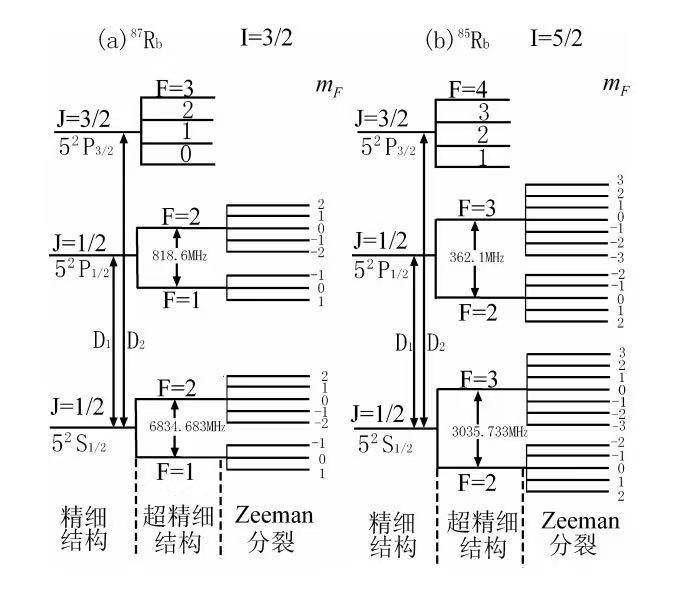
\includegraphics[width=15cm,height=10cm]{textlevel}
    \caption{铷原子的能级结构示意图}
    \label{key}
\end{figure}

在弱磁场条件下，通过求解 Rb 原子的定态薛定谔方程，其能量本征值可写为
\begin{equation}
    E = E_0 + \frac{ah}{2}\!\left[F(F+1)-J(J+1)-I(I+1)\right] + g_F m_F \mu_B B_0 ,
\end{equation}
由此可以得到以下两个重要结果：
\begin{itemize}
    \item \textbf{相邻超精细能级之间的能量差}
    \begin{equation}
        \Delta E_F = \frac{ah}{2}\left[F'(F'+1)-F(F+1)\right] ;
    \end{equation}
    \item \textbf{相邻塞曼子能级之间的能量差}
    \begin{equation}
        \Delta E_{m_F} = g_F \mu_B B_0 .
    \end{equation}
\end{itemize}

\subsection{光抽运效应的物理过程}

在原子与光相互作用的过程中，能级跃迁需满足严格的选择定则。对磁量子数而言，这些定则尤为关键，因为跃迁过程中吸收或辐射的光子携带角动量，其自旋角动量的取向与光的偏振状态直接相关\footnote{圆偏振光具有自旋角动量，左旋 $\sigma^+$ 光的角动量为 $\hbar$，右旋 $\sigma^-$ 光的角动量为 $-\hbar$}。

在热平衡状态下，基态各塞曼子能级上的原子数服从玻尔兹曼分布 $N \sim \exp(-\beta E)$。由于弱磁场中相邻塞曼子能级的能量差极小，可以近似认为原子在各子能级上的分布是均匀的。光抽运的核心目的正是打破这种均匀分布，使原子数在磁子能级之间产生明显的偏极化。

具体而言，当左旋（或右旋）圆偏振光照射原子体系时，选择定则仅允许 $\Delta m_F = +1$（或 $\Delta m_F = -1$）的跃迁发生。以左旋圆偏振光为例，基态中 $m_F = +2$ 的子能级将无法被进一步激发，而处于激发态的原子在自发辐射和无辐射跃迁过程中，以近似相等的概率回到基态的各个子能级。经过一段时间后，原子将逐渐积聚在 $5^2S_{1/2}$ 态的 $m_F=+2$ 子能级上，从而形成显著的粒子数偏极化，这一过程即称为\textbf{光抽运效应}。为抑制非平衡态向平衡态的弛豫，实验中通常引入缓冲气体，并通过控制工作温度来增强共振信号。

在外磁场刚施加的瞬间，基态各 Zeeman 子能级上的粒子数仍近似均匀，此时约有总粒子数的 $7/8$ 能够吸收 $D_1$ 线的 $\sigma^+$ 光，吸收最为强烈。随着光抽运过程的进行，越来越多的原子被转移到 $m_F=+2$ 子能级，能够吸收光的原子数随之减少，透射光强逐渐增强。当该子能级达到饱和占据时，透射光强达到最大。若扫场方波经过零点并反向，Zeeman 子能级将发生简并并重新分裂，在简并阶段原子由于碰撞而失去偏极化；再次分裂后，各子能级上的粒子数重新趋于均匀，对 $D_1$ 光的吸收再次增强，从而在探测信号中形成明显的\textbf{光抽运信号}。

\subsection{Zeeman 子能级之间的磁共振}

在恒定磁场 $\bm{B}_0$ 的垂直方向上施加角频率为 $\omega_1$ 的线偏振射频磁场 $\bm{B}_1$。该射频磁场可分解为一对左旋和右旋的圆偏振磁场。当 $g_F>0$ 时，原子磁矩 $\bm{\mu}_F$ 作右旋进动，真正参与相互作用的是右旋分量
\[
\bm{B}_1 = B_1\!\left(\cos(\omega_1 t)\bm{e}_x + \sin(\omega_1 t)\bm{e}_y\right) .
\]
当射频场频率满足共振条件
\begin{equation}\label{B_0}
    \hbar \omega_1 = \Delta E_{m_F} = g_F \mu_B B_0 ,
\end{equation}
相邻 Zeeman 子能级之间便会发生磁共振跃迁。原本被光抽运聚集在基态 $m_F=+2$ 子能级上的原子，在射频磁场作用下跃迁至 $m_F=+1$ 子能级；与此同时，光抽运过程仍持续进行，将其他子能级上的原子重新抽运回 $m_F=+2$。当磁共振与光抽运达到动态平衡时，$m_F=+2$ 子能级的粒子数下降，其余子能级粒子数上升，对 $D_1$ 光的吸收显著增强，导致探测光强骤然减小，这一现象即为\textbf{磁共振信号}。

\subsection{仪器原理}

\subsubsection{偏振光的获取}

自然光经偏振片起偏后进入波晶片，在晶体中分解为偏振方向相互正交的普通光（o 光）和非普通光（e 光），二者因折射率不同而产生相位差。选用四分之一波片并使其光轴与起偏器透振方向成 $45^\circ$，即可引入 $\pi/2$ 的相位差，使出射光转化为圆偏振光。

\subsubsection{磁场的控制}

实验中采用亥姆霍兹线圈系统产生所需磁场，包括水平线圈、垂直线圈、扫场线圈以及射频线圈。水平线圈的轴线应尽量与地磁场的水平分量方向一致；垂直线圈用于补偿地磁场的竖直分量，以获得最佳共振条件。扫场磁场既可采用方波形式，也可采用三角波形式，并与示波器的扫描信号保持同步。射频磁场由信号发生器提供，本实验选用的频率为实验推荐值。

实验装置中，两个水平线圈采用并联连接，电流表显示的是流经两线圈的总电流；两个垂直线圈则为串联连接，电流表读数对应单个线圈的电流。水平与垂直线圈产生的磁场强度分别为
\begin{align}
    B_{\text{水平}} &= \frac{16\pi}{5^{3/2}}\frac{N}{r} I \times 10^{-3} , \label{hor}\\
    B_{\text{垂直}} &= \frac{32\pi}{5^{3/2}}\frac{N}{r} I \times 10^{-3} , \label{ver}
\end{align}
其中 $N$ 为每个线圈的匝数，$r$ 为线圈的有效半径（单位 m），$I$ 为线圈电流（单位 A），$B$ 的单位为 Gs。

扫场线圈输出的方波信号可表示为围绕偏置磁场的周期性扰动，在一个周期内分别取 $B_1+\Delta B_1$ 与 $B_1-\Delta B_1$；三角波信号则在 $B_2+\Delta B_2$ 与 $B_2-\Delta B_2$ 之间线性变化。前者用于光抽运信号的观测，后者用于磁共振信号的测量。

    \section{实验}
    
        \subsection{实验仪器}
\subsubsection{Rb原子光谱灯与样品泡}
铷原子光谱灯采用高频无极放电 Rb 灯作为光源。样品泡为直径约 5\,cm 的玻璃泡，内部充有适量天然铷蒸汽，并加入约 10\,Torr 的氮气和氩气作为缓冲气体。样品泡放置于恒温装置中工作，其温度对实验信号具有显著影响。当温度升高时，铷蒸汽原子密度增大，原子间以及原子与器壁之间的碰撞频率增加，从而削弱原子的偏极化程度；而当温度过低时，原子数密度不足，会导致探测到的信号幅度明显减小。综合考虑上述因素，实验中将样品泡温度控制在 $40\text{--}60\,^\circ\mathrm{C}$ 范围内，且温度波动不超过 $\pm 1\,^\circ\mathrm{C}$。同时，将 Rb 灯温度维持在约 $90\,^\circ\mathrm{C}$，以保证足够的光强并获得清晰的共振信号。
\subsubsection{圆偏振光发生器}
偏振片与四分之一波片组合使用，用于将入射的自然光转化为圆偏振光，从而满足光抽运过程对光偏振态的要求。
\subsubsection{干涉滤光片与透镜组}
在光路中引入干涉滤光片，其透过率大于 $60\%$，带宽小于 15\,nm。该滤光片的作用在于有效抑制不利于光抽运过程的 $\mathrm{D}_2$ 线，仅保留 $\mathrm{D}_1$ 线参与相互作用。由于 $\mathrm{D}_1$ 与 $\mathrm{D}_2$ 两条谱线的波长差约为 15\,nm，该滤光方案能够较好地实现谱线分离。

为提高光电探测器接收到的信号强度，实验中采用两片透镜对光束进行整形与聚焦。透镜 $L_1$ 用于将光源发出的发散光近似准直，而透镜 $L_2$ 则将通过样品泡后的平行光会聚到光电探测器的有效接收区域内，从而提高信噪比。
\subsubsection{场信号发生器}
实验所需磁场由亥姆霍兹线圈产生。通过调节线圈中电流的大小与方向，可以分别控制稳恒磁场及扫场磁场的强度与方向。

射频信号由信号发生器提供，用于在磁共振实验中激发铷原子的磁共振跃迁。
\subsubsection{信号探测与显示}
光信号的探测由光电探测器完成，其由光电接收元件及后级放大电路组成。光电接收元件可选用光电管或光电池。光电管具有响应速度快的优点，而光电池虽响应时间较长，但其受光面积大、内阻低，更适合本实验的信号检测需求，因此实验中选用光电池作为探测元件。

示波器用于实时显示光抽运信号以及磁共振信号，是观察和记录实验现象的主要工具。

\begin{figure}[h!]
        \centering
        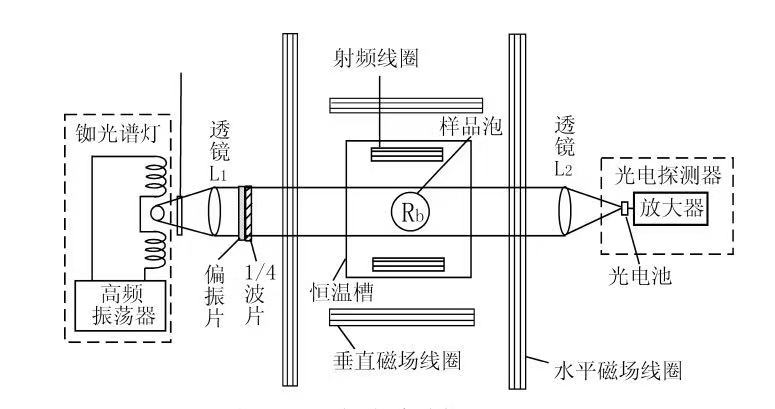
\includegraphics[width=12cm,height=6cm]{lightway}
        \caption{实验光路示意图}
        \label{key}
    \end{figure}

\subsection{实验操作及主要内容}

实验开始前需对整套装置进行预热，以确保样品泡与 Rb 灯工作在稳定温度条件下。预热时间约为半小时，当“灯温”和“池温”指示达到设定状态后，即可进行后续实验操作。

光路调节是实验中的关键步骤之一。首先对光学元件进行粗略调整，使其大致处于等高、共轴状态；随后结合示波器上显示的信号强度，对偏振片角度、透镜位置等参数进行细致调整，以获得尽可能强且稳定的信号。

由于实验初始阶段无法直接判断各线圈所产生磁场的方向，需要对磁场方向进行逐一确认。通过改变扫场线圈中电流的方向并观察光抽运信号的变化，可以确定其磁场方向与地磁场水平分量之间的相对关系；随后采用类似方法判断垂直线圈和水平线圈所产生磁场的方向。

在明确各磁场方向后，向垂直线圈中通入适当电流，用以补偿地磁场的垂直分量。当垂直方向的总磁场接近零时，光抽运信号达到最大。此时将扫场线圈设置为方波输出，并调节水平线圈中的电流大小。在合适的参数条件下，方波反转时刻附近会出现明显的信号跃变。通过调整水平线圈电流，使一个周期内出现的两次跃变幅度相等，即可认为水平磁场与地磁场水平分量实现抵消。

磁共振信号的测量采用扫场法完成。实验中保持射频磁场频率不变，通过改变稳恒磁场的大小来满足共振条件。将扫场线圈设为三角波输出，在一定电流范围内，可以观察到信号在三角波周期内的特定位置发生跃变，对应磁共振的出现。记录跃变出现时对应的电流值，即可用于后续数据分析。


    \section{结果与分析讨论}
       \subsection{光抽运信号}

\begin{figure}[h!]
    \centering
    \begin{subfigure}{0.3\textwidth}
        \centering
        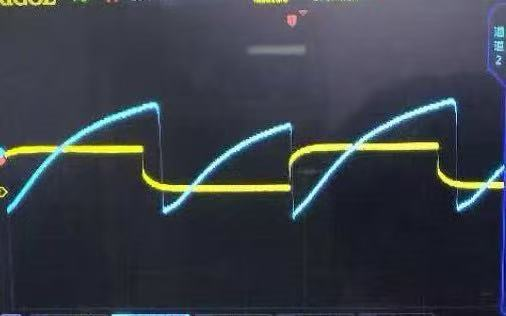
\includegraphics[width=\textwidth,height=3cm]{low}
        \caption{水平线圈电流偏低，地磁场水平分量未完全抵消的光抽运信号}
        \label{fig:low_current}
    \end{subfigure}
    \hfill
    \begin{subfigure}{0.3\textwidth}
        \centering
        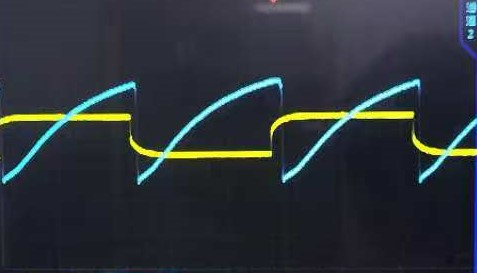
\includegraphics[width=\textwidth,height=3cm]{proper}
        \caption{水平线圈电流适中，地磁场水平分量刚好被抵消的光抽运信号}
        \label{fig:proper_current}
    \end{subfigure}
    \hfill
    \begin{subfigure}{0.3\textwidth}
        \centering
        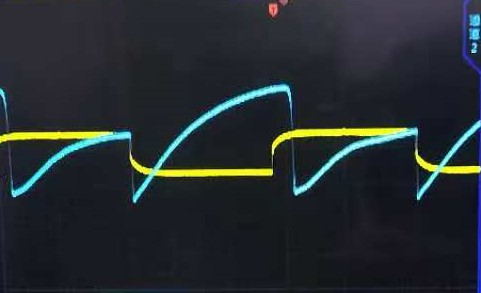
\includegraphics[width=\textwidth,height=3cm]{surpass}
        \caption{水平线圈电流偏高，地磁场水平分量被过度抵消的光抽运信号}
        \label{fig:high_current}
    \end{subfigure}
    \caption{随着水平线圈电流变化，光抽运信号的不同表现}
    \label{fig:optical_pumping}
\end{figure}

当水平线圈电流略低于或略高于抵消地磁场水平分量所需电流时，虽然仍能观测到光抽运信号，但信号在一个周期内呈现不对称状态。通过进一步调节水平线圈电流，信号可达到最大值，记录的电流数据如下：

\begin{table}[h!]
    \centering
    \caption{光抽运信号测量数据}
    \label{tab:optical_data}
    \begin{tabular}{|c|c|c|c|c|}
    \hline
         & 扫场方向 & 水平方向 & 水平电流 (mA) & 垂直电流 (mA) \\
    \hline
    \multirow{2}{*}{A} & - & - & 0.020 & \multirow{2}{*}{0.067} \\
    \cline{2-4}
         & + & - & 0.097 &  \\
    \hline
    \multirow{2}{*}{B} & - & + & 0.130 & \multirow{2}{*}{0.067} \\
    \cline{2-4}
         & + & - & 0.228 &  \\
    \hline
    \multirow{2}{*}{C} & - & + & 0.170 & \multirow{2}{*}{0.067} \\
    \cline{2-4}
         & + & - & 0.282 &  \\
    \hline
    \end{tabular}
\end{table}

各次测量中垂直电流相同，代入公式 (\ref{ver}) 得到地磁场垂直分量：
\[
B_{\text{垂直}} = 0.39376\ \text{Gs}.
\]

根据三组水平电流数据，代入公式 (\ref{hor}) 得到地磁场水平分量：
\[
\begin{aligned}
B_{\text{水平}}^A &= 0.27477\ \text{Gs},\\
B_{\text{水平}}^B &= 0.23015\ \text{Gs},\\
B_{\text{水平}}^C &= 0.26303\ \text{Gs}.
\end{aligned}
\]

取平均值得：
\[
B_{\text{水平}} = \frac{0.27477 + 0.23015 + 0.26303}{3} \approx 0.25598\ \text{Gs}.
\]

磁倾角计算如下：
\[
\theta = \arctan\frac{B_{\text{垂直}}}{B_{\text{水平}}} = 56.97^\circ.
\]

\textbf{误差分析}
\begin{enumerate}
    \item 判断两次跃变幅度是否相等时，示波器未调整显示比例，导致水平电流读数存在较大不确定度，进而影响地磁场水平分量测量精度；
    \item 水平线圈轴线可能未严格与地磁场水平分量平行，实际测量值可能仅为水平分量的投影，导致读数偏小。
\end{enumerate}

\subsection{磁共振信号}

\begin{figure}[h!]
    \centering
    \begin{subfigure}{0.47\textwidth}
        \centering
        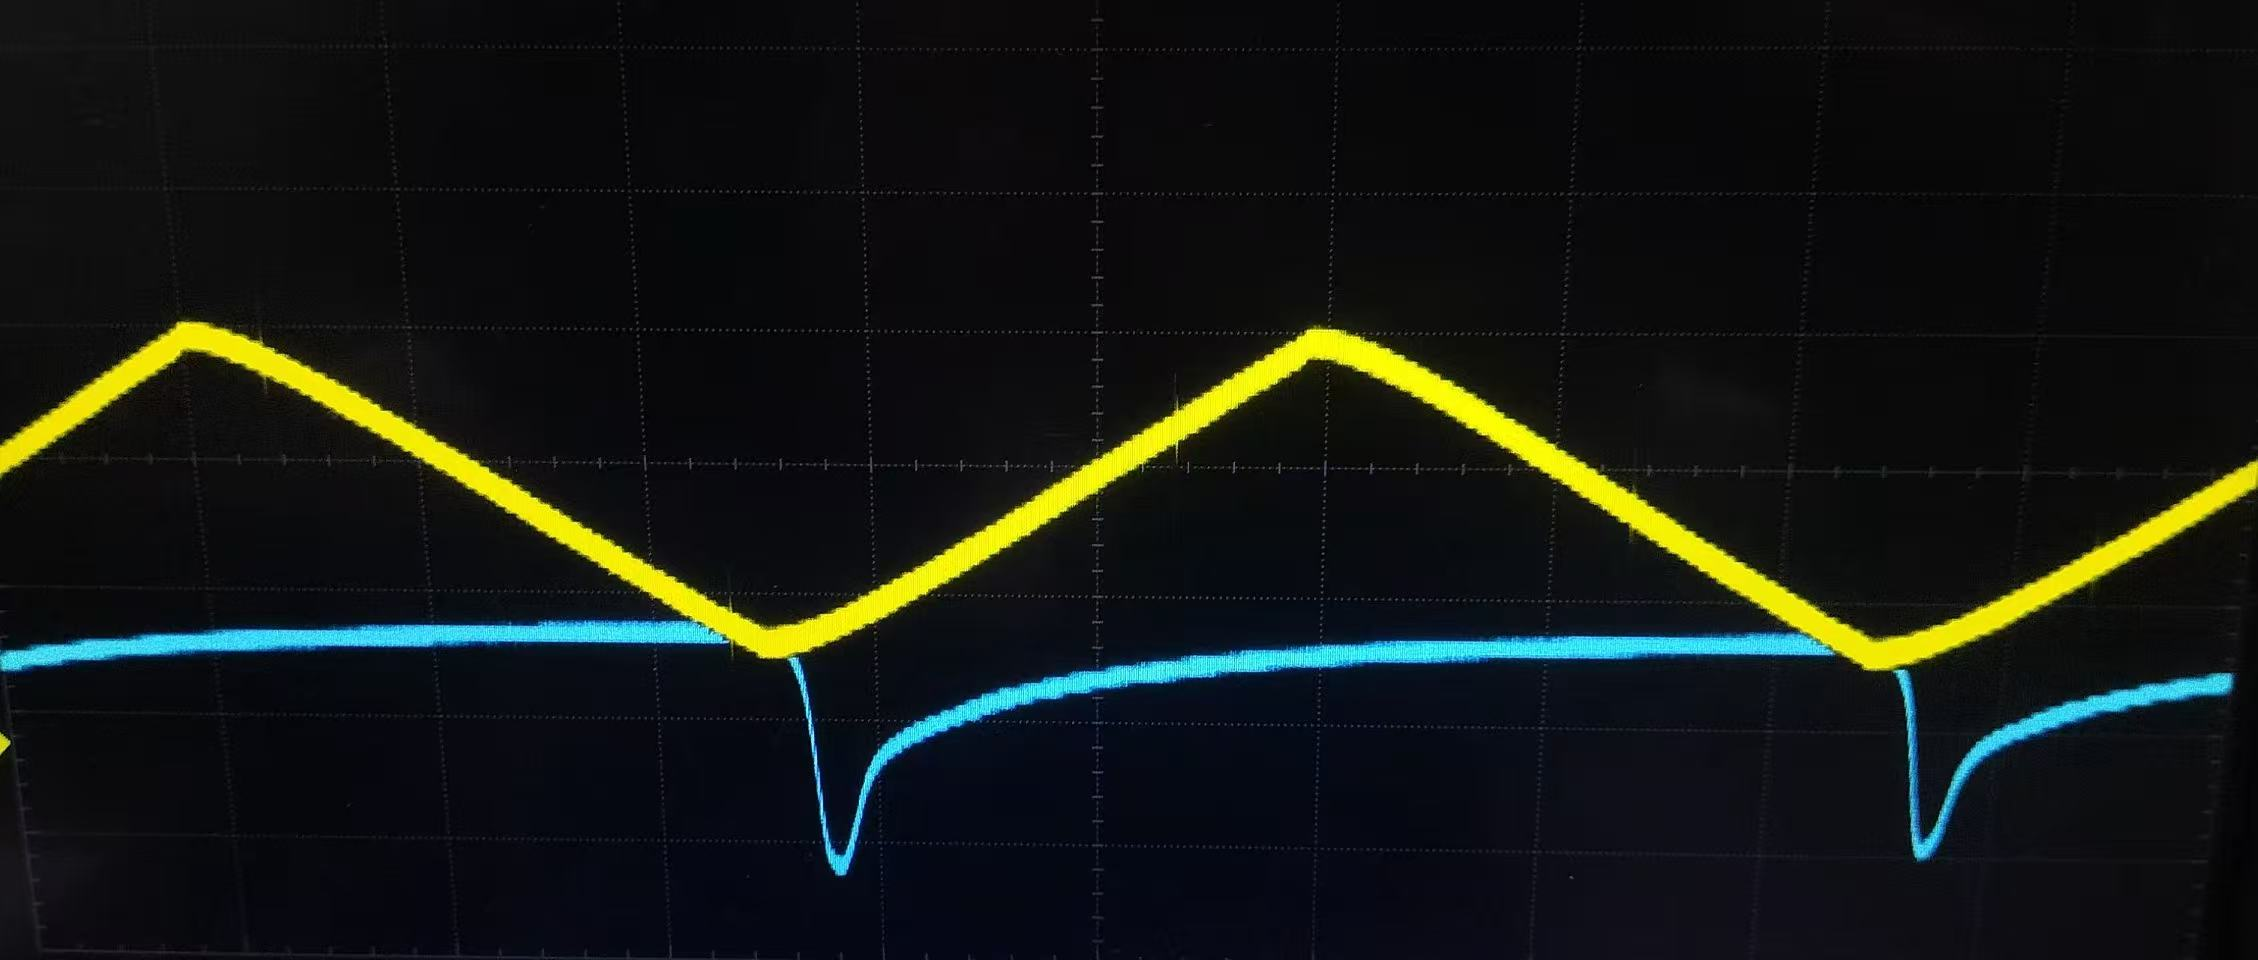
\includegraphics[width=\textwidth,height=4cm]{mag}
        \caption{波谷共振信号}
        \label{fig:resonance_valley}
    \end{subfigure}
    \hfill
    \begin{subfigure}{0.47\textwidth}
        \centering
        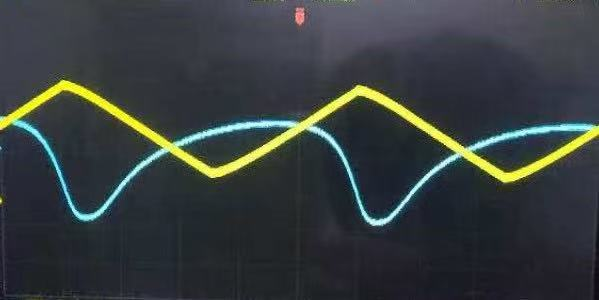
\includegraphics[width=\textwidth,height=4cm]{pseudo}
        \caption{赝磁共振信号示意}
        \label{fig:pseudo_resonance}
    \end{subfigure}
    \caption{磁共振信号示意图}
    \label{fig:mag_resonance}
\end{figure}

当信号发生器输出频率时，若地磁场水平分量、水平线圈磁场及扫场线圈磁场的合成磁场满足磁共振条件，可在示波器上观测到真实的磁共振信号。但在总磁场可能过零的情况下，也可能出现赝磁共振信号。

实验测量了不同扫场方向及水平、垂直线圈电流组合下的磁共振信号对应的电流范围，数据如下：

\begin{table}[h!]
    \centering
    \caption{磁共振信号测量数据}
    \label{tab:resonance_data}
    \begin{tabular}{|c|c|c|c|c|c|}
    \hline
    扫场方向 & 水平方向 & $I_1$ & $I_2$ & $I_3$ & $I_4$ \\
    \hline
    + & + & 79 & 123 & 176 & 219 \\
    - & + & 178 & 223 & 276 & 321 \\
    + & - & 276 & 322 & 373 & 420 \\
    - & - & 173 & 218 & 272 & 317 \\
    \hline
    \end{tabular}
\end{table}

其中 $I_1$、$I_2$ 为 $^{87}\mathrm{Rb}$ 磁共振下界和上界电流，$I_3$、$I_4$ 为 $^{85}\mathrm{Rb}$ 磁共振下界和上界电流。根据附录公式计算得：

\begin{itemize}
    \item $^{87}\mathrm{Rb}$：波峰 $g = 0.4962$，波谷 $g = 0.4975$，取平均 $g \approx 0.497$；
    \item $^{85}\mathrm{Rb}$：波峰 $g = 0.3326$，波谷 $g = 0.3329$，取平均 $g \approx 0.333$。
\end{itemize}

地磁场水平分量为：
\[
B_{\text{水平}} = \frac{I_1 + I_2 + I_3 + I_4}{4} \approx 0.249\ \text{Gs}.
\]

磁倾角：
\[
\theta = \arctan\frac{B_{\text{垂直}}}{B_{\text{水平}}} = 57.73^\circ.
\]

\textbf{误差分析}
\begin{enumerate}
    \item 磁共振信号在出现瞬间通常不稳定，导致水平线圈电流测量存在误差；
    \item 射频信号方向可能未严格垂直于水平磁场；
    \item 实验室内其他磁场干扰可能影响地磁场测量。
\end{enumerate}

    \section{总结}
        在实验过程中，我们观察了在不同电流条件下光抽运信号的变化，并由此估算了地磁场的垂直分量和水平分量。实验结果显示，光抽运信号随水平线圈电流的调整呈现出规律性的变化，这为地磁场分量的测定提供了可靠依据。

在磁共振实验中，通过测量不同同位素的朗德因子，可以发现实验值与理论预期非常接近，说明光泵磁共振方法在测量磁场及原子物理参数方面具有较高的精度。多次实验的结果表明，地磁场水平分量的测定具有良好的重复性和稳定性。

    \begin{thebibliography}{99}
        \bibitem{1}
        北京师范大学物理实验教学中心. 近代物理实验讲义一 (2019)
    \end{thebibliography}

    
\end{document}